\documentclass[preprint,12pt]{elsarticle}
\usepackage[utf8]{inputenc}
\usepackage[T1]{fontenc}
\usepackage{amsmath,amssymb}
\usepackage{booktabs}
\usepackage{xcolor}
\usepackage{listings}
\usepackage{pgfplots}
\usepackage[hidelinks]{hyperref}
\pgfplotsset{compat=1.18}
\usetikzlibrary{positioning}
\lstset{basicstyle=\ttfamily\small,columns=fullflexible,keepspaces=true,
        frame=single,framerule=0.3pt,xleftmargin=2pt,xrightmargin=2pt}
\newcommand{\authors}[1]{\textcolor{red}{[AUTHORS: #1]}}
\input{gen/numbers.tex}
\journal{SoftwareX}

\begin{document}
\begin{frontmatter}

\title{logq: integer-only binary logarithms with verified error bounds for processors without a floating-point unit}

\author[usc]{Ewa Deelman\corref{cor}}
\ead{deelman@isi.edu}
\author[pw]{Pawel Gepner}
\author[pw]{Leonid Moroz}
\author[pk]{Pawel Poczekajlo}
\cortext[cor]{Corresponding author}
\address[usc]{University of Southern California, Information Sciences Institute, Marina del Rey, 90292, CA, USA}
\address[pw]{Warsaw University of Technology, Faculty of Mechanical and Industrial Engineering, 02-524 Warszawa, Poland}
\address[pk]{Koszalin University of Technology, Faculty of Electronics and Computer Science, 75-453, Koszalin, Poland}

\begin{abstract}
Small processors without a floating-point unit compute logarithms for sound
levels, spectral features, entropies and logarithmic number systems, yet the
C library \texttt{log2f} costs them 1500--3500 instructions of emulated
floating point. logq is a header-only C99 library and a generator that produce
binary logarithms using integer operations only. A family of piecewise minimax
polynomials, tunable in degree and number of segments, returns log$_2$ in
fixed point with a guaranteed absolute error between \numEmax{} and
\numEmin{}; a second family bounds the relative error, down to 0.54~ulp of
binary32. The generator verifies every variant it emits on all $2^{23}$
significands, and the test suite checks every positive binary32 input. \authors {On
RV32IM and Cortex-M0 a full-domain binary32 logarithm takes \numinsmin--\numinsmax{}
instructions, \numratmin--\numratmax{} times fewer than \texttt{log2f}.}
On an ESP32-C3 microcontroller (RV32IMC) the fixed-point logarithm takes 65
clock cycles, against 3430 for the \texttt{log2f} of the toolchain's C library.
\end{abstract}

\begin{keyword}
logarithm \sep fixed-point arithmetic \sep microcontroller \sep RISC-V \sep Cortex-M \sep exhaustive verification
\end{keyword}
\end{frontmatter}

\section*{Code metadata}
{\small
\begin{tabular}{p{0.06\linewidth}p{0.42\linewidth}p{0.44\linewidth}}
\toprule
Nr. & Code metadata description & Metadata \\
\midrule
C1 & Current code version & v1.0.0 \\
C2 & Permanent link to code/repository used for this code version & \url{https://github.com/pawelgepner/Logarithm} \\
C3 & Permanent link to Reproducible Capsule & \authors{optional, e.g.\ Code Ocean capsule} \\
C4 & Legal Code License & MIT \\
C5 & Code versioning system used & git \\
C6 & Software code languages, tools, and services used & C99, Python 3 (NumPy); CMake; clang/lld and Unicorn for the emulated benchmarks; ESP-IDF for the hardware benchmark; GitHub Actions \\
C7 & Compilation requirements, operating environments \& dependencies & Any C99 compiler; no run-time dependencies. Generator: Python $\ge$3.8 with NumPy. Benchmarks: clang with RISC-V and Arm targets, LLVM compiler-rt sources, Python package \texttt{unicorn}; ESP-IDF 5.x for the ESP32-C3 benchmark \\
C8 & If available Link to developer documentation/manual & \url{https://github.com/pawelgepner/Logarithm\#readme} \\
C9 & Support email for questions & pawel.gepner@pw.edu.pl \\
\bottomrule
\end{tabular}}

\section{Motivation and significance}

Many embedded processors have no floating-point unit: RV32I/RV32IM cores,
Arm Cortex-M0, M0+ and M3, and most low-cost microcontrollers. Their
programs nevertheless need logarithms. A sound-level meter reports decibels;
keyword spotting on microcontrollers starts from log-mel spectral features
\cite{zhang2017helloedge}; estimators compute entropies and log-likelihoods;
logarithmic number systems replace multiplication by addition of
fixed-point logarithms \cite{coleman2000}. On such cores the C library
function \texttt{log2f} runs on software-emulated floating point.
Table~\ref{tab:cost} shows what this costs: 1548 instructions on RV32IM and
3154 on Cortex-M0 for the Arm Optimized Routines implementation used by musl
and glibc \cite{aor}, more for the fdlibm-derived one \cite{freebsdmsun}.
These functions are also more accurate than most such applications need.

Two other options exist. Fixed-point libraries offer logarithms of fixed
accuracy: CMSIS-DSP computes the natural logarithm of a Q31 number bit by bit,
with 31 iterations of Turner's algorithm \cite{cmsisdsp,turner2010}. Hardware
and software approximations derived from Mitchell's method
\cite{mitchell1962} are cheap, but their error is usually stated for sampled
inputs, if at all. At the other end, correctly rounded libraries such as
CORE-MATH and RLIBM \cite{sibidanov2022coremath,lim2021rlibm32} give the
strongest guarantee but assume floating-point hardware.

logq fills the space between these options. The user chooses the accuracy;
the generator emits integer-only C code for it and proves its worst-case
error by evaluating the emitted integer kernel on every possible significand.
The library grew out of the algorithms in our 2023 preprint
\cite{gepner2023preprint}, kept unchanged in the repository under the tag
\texttt{v0.1-preprint}. That version used floating-point operations,
did not handle subnormal numbers, zeros or special values, reported errors for
sampled inputs, and its benchmark timed a single constant argument. Version
1.0 is a new implementation that removes each of these limitations, and it
does not reproduce the speed-ups over desktop C libraries reported there:
on processors with hardware floating point, \texttt{log2f} remains faster.

\section{Software description}

\subsection{Software architecture}

logq has three parts (Fig.~\ref{fig:arch}):
\begin{itemize}
\item \texttt{tools/logqgen.py}, the generator, which computes the
  coefficients of a variant, verifies the resulting integer code and emits a
  self-contained C99 header;
\item \texttt{include/logq.h}, the generated catalogue of all
  \numnvariants{} absolute-error and 15 relative-error variants, for users who
  do not want to run the generator;
\item the verification and benchmark suite in \texttt{tests/} and
  \texttt{bench/}, which re-checks the headers independently of the generator
  and measures their cost on emulated FPU-less cores and, with the ESP-IDF
  project in \texttt{bench/hw/esp32c3}, on a real microcontroller.
\end{itemize}

\begin{figure}[t]
\centering
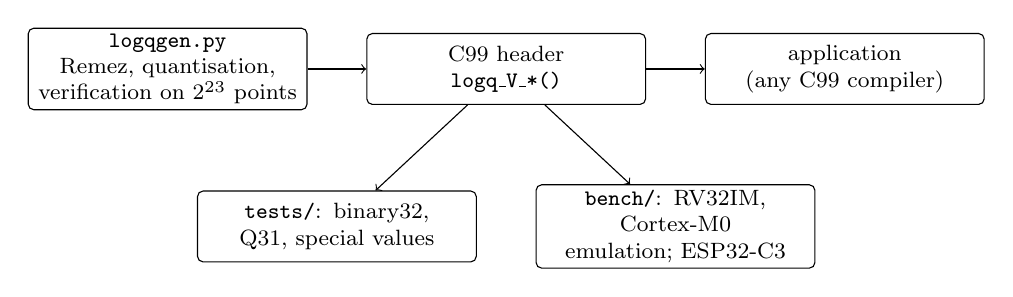
\begin{tikzpicture}[font=\footnotesize,
  box/.style={draw, rounded corners=2pt, align=center, minimum height=9mm, inner sep=2pt, text width=34mm}]
\node[box] (g) at (0,0) {\texttt{logqgen.py}\\Remez, quantisation,\\verification on $2^{23}$ points};
\node[box] (h) at (4.3,0) {C99 header\\\texttt{logq\_V\_*()}};
\node[box] (a) at (8.6,0) {application\\(any C99 compiler)};
\node[box] (t) at (2.15,-2.0) {\texttt{tests/}: binary32,\\Q31, special values};
\node[box] (b) at (6.45,-2.0) {\texttt{bench/}: RV32IM, Cortex-M0\\emulation; ESP32-C3};
\draw[->] (g) -- (h); \draw[->] (h) -- (a); \draw[->] (h) -- (t); \draw[->] (h) -- (b);
\end{tikzpicture}
\caption{Components of logq.}
\label{fig:arch}
\end{figure}

\subsection{Algorithms}

A positive binary32 number is $x = 2^{e}(1+m)$ with $m = k/2^{23}$, so
$\log_2 x = e + \log_2(1+m)$. Subnormal inputs are normalised with a
count-leading-zeros instruction, and the same path serves 32-bit integer
inputs. The kernel approximates $\log_2(1+m)$ on $p$ segments of $[0,1)$ by a
polynomial of degree $n$:

\textbf{Family A$(n,p,\sigma)$} uses uniform ($\sigma=\mathrm{u}$) or
geometric ($\sigma=\mathrm{g}$, boundaries $2^{j/p}-1$) segments. The segment
index is the top $\log_2 p$ bits of $k$ for uniform segments and a binary
search over $p$ boundaries for geometric ones. The polynomial is
evaluated by Horner's rule on the offset $t$ of $k$ within its segment, with
Q30 coefficients, 32-bit operands and 64-bit products. The result is rounded
once to Q23 and added to $e\cdot2^{23}$, which gives $\log_2 x$ in Q8.23
fixed point. Its error is exactly the kernel error, so the bound verified by
the generator holds for every input. If a binary32 result is requested, it is
packed with round-to-nearest-even by integer operations, and the error grows
by at most half an ulp of the result.

\textbf{Family R$(n,p)$} removes the weakness of family A near $x=1$, where
$\log_2 x \to 0$ and a fixed absolute error becomes an unbounded relative
error. It writes $\log_2(1+z) = z\,q(z)$ with $q(z)=\log_2(1+z)/z$, takes
$z=m$ for $m<\sqrt2-1$ and $z=(m-1)/2$ with $e+1$ otherwise, approximates
$q$ by the same piecewise scheme, and forms $e+z\,q(z)$ in 64-bit fixed point
before a single rounding to binary32. The result is exact at all powers of two
and has a bounded relative error. With 32 segments it matches the binary32
\texttt{log2f} of Arm Optimized Routines, the implementation used by musl and
glibc \cite{aor}: \texttt{R3\_32} returns the same result for 99.98\% of all
positive binary32 inputs and differs by one ulp for the remaining 405\,402,
while using integer operations only.

\subsection{Generator and verification}

For each segment the generator computes the minimax polynomial by the Remez
exchange algorithm \cite{muller2016}, rounds the coefficients to Q30 and
evaluates the resulting \emph{integer} code on every significand of the
segment. It then recentres the constant term on the observed error and
re-verifies. The reported bound is therefore a property of the emitted code,
including quantisation and rounding, not of the real-valued polynomial.
Fig.~\ref{fig:err} shows the bounds: the error falls as $p^{-(n+1)}$ until it
reaches the Q23 output resolution. Geometric segments equalise the error
across segments and reduce it two to three times for the same $p$, at the
price of the binary search. Doubling $p$ with uniform segments is usually the
better trade: \texttt{A2\_32u} has a smaller error than \texttt{A2\_16g}
(\numeAtwou{} against \numeAsixg) and costs fewer instructions
(\numiAtwou{} against \numiAsixg{} on RV32IM, \nummAtwou{} against \nummAsixg{} on
Cortex-M0), so geometric segments pay off only when table memory is tight.

\begin{figure}[t]
\centering
\begin{tikzpicture}
\begin{loglogaxis}[width=0.62\linewidth, height=6.2cm, xlabel={segments $p$},
  ylabel={max.\ $|$error$|$ of $\log_2$ (kernel)}, log basis x=2,
  xtick={1,2,4,8,16,32,64}, legend pos=outer north east, legend style={font=\scriptsize},
  grid=major, grid style={gray!25}]
\addplot[blue, mark=*] table {gen/err_n1u.dat}; \addlegendentry{$n=1$, uniform}
\addplot[blue, dashed, mark=o] table {gen/err_n1g.dat}; \addlegendentry{$n=1$, geometric}
\addplot[red, mark=square*] table {gen/err_n2u.dat}; \addlegendentry{$n=2$, uniform}
\addplot[red, dashed, mark=square] table {gen/err_n2g.dat}; \addlegendentry{$n=2$, geometric}
\addplot[black, mark=triangle*] table {gen/err_n3u.dat}; \addlegendentry{$n=3$, uniform}
\addplot[black, dashed, mark=triangle] table {gen/err_n3g.dat}; \addlegendentry{$n=3$, geometric}
\addplot[gray, thin, domain=1:64] {2^(-24)}; \addlegendentry{$2^{-24}$ (half Q23 unit)}
\end{loglogaxis}
\end{tikzpicture}
\caption{Verified worst-case kernel error of the family-A variants, from \texttt{results/kernel\_exhaustive.csv}.}
\label{fig:err}
\end{figure}

The test suite re-checks the generated headers independently:
\texttt{test\_kernel} repeats the $2^{23}$-point check in C and tests
monotonicity across binades; \texttt{test\_float} evaluates all 54 variants
on every positive finite binary32 number ($2.14\times10^{9}$ inputs) and
checks that each family-A result lies within the kernel bound plus half an
ulp, which holds for all \numnvariants{} variants; \texttt{test\_special}
covers zeros, infinities, NaNs and extreme values, the exactness of family R
at powers of two, and the integer entry point for all $2^{32}-1$ integers.
\numnmono{} of the \numnvariants{} family-A variants are monotonic; the
exceptions are the linear uniform variants with $p\ge2$ and two cubic ones, whose error
steps at segment boundaries. \texttt{tools/check\_generated.py} confirms that
the committed tables are reproduced bit for bit by the generator, and all
tests run in continuous integration.

\subsection{Software functionalities}

For a family-A variant \texttt{V} the header provides
\texttt{logq\_V\_kernel(k)} ($\log_2(1+k/2^{23})$ in Q23),
\texttt{logq\_V\_q23(bits)} (Q8.23 result for a normal binary32 bit pattern),
\texttt{logq\_V\_q23\_u32(v)} (Q8.23 result for an integer $v\ge1$) and
\texttt{logq\_V\_f32bits}/\texttt{logq\_V\_f32} (binary32 over the full IEEE
754 domain). Family R provides the last two. No function executes a
floating-point operation; arguments and results can travel as bit patterns,
so the code also runs where the compiler's soft-float library is absent.
For \texttt{A2\_16u} the kernel alone takes \numkernrv/\numkernmz{}
instructions on RV32IM/Cortex-M0, the fixed-point result from a binary32
\numfixrv/\numfixmz{}, and from an integer \numintrv/\numintmz.

\section{Illustrative examples}

\subsection{Choosing and generating a variant}
A product usually needs one variant. The command
\begin{lstlisting}
$ python3 tools/logqgen.py -n 2 -p 4 --seg g --prefix mylog_ -o mylog.h
A2_4g  tables 64 B  minimax 7.813e-05  verified [-7.819e-05, +7.819e-05]
\end{lstlisting}
writes a header with 64 bytes of tables and reports the verified bound. The
difference between the minimax error and the verified error is the cost of
integer evaluation; it becomes visible below $10^{-6}$ (Fig.~\ref{fig:err}).

\subsection{Sound level of PCM frames}
\texttt{examples/db\_meter.c} computes the level in dBFS of 256-sample
16-bit frames with integers only:
\begin{lstlisting}[language=C]
while (e >> 32) { e >>= 1; sh++; }      /* 32 leading bits of the energy */
int32_t l2 = logq_A2_16u_q23_u32((uint32_t)e) + ((sh - 8 - 30) << 23);
return (int32_t)(((int64_t)l2 * TEN_LOG10_2_Q28) >> 28);   /* dB, Q8.23 */
\end{lstlisting}
Over 10\,000 synthetic frames the result differs from double precision by at
most $1.1\cdot10^{-5}$~dB, as predicted by the bound of \texttt{A2\_16u}
($3.4\cdot10^{-6}$ in $\log_2$, plus truncation of the energy).

\subsection{Cost and accuracy against existing implementations}
Table~\ref{tab:cost} compares full-domain binary32 logarithms. Instruction
counts come from running each function in the Unicorn emulator
\cite{unicorn}, cross-compiled with clang~18 at \texttt{-O2} against the LLVM
compiler-rt soft-float routines \cite{compilerrt}, on 1000 log-uniform
inputs; every emulated result is compared bit for bit with the same function
compiled for the host. The footprint is the size of a bare-metal image that
contains only that function and everything it calls. The accuracy of all
functions was measured on every positive binary32 input.

\begin{table}[t]
\centering\small
\caption{Full-domain binary32 $\log_2$: worst-case error over all positive
binary32 inputs and mean executed instructions (1000 inputs). Absolute error
excludes the final rounding to binary32 (at most half an ulp).}
\label{tab:cost}
\begin{tabular}{@{}lllrrr@{}}
\toprule
Function & Abs.\ error & Rel.\ error & RV32IM & Cortex-M0 & Bytes (M0) \\
\midrule
\csname @@input\endcsname gen/tab_cost.tex
\bottomrule
\end{tabular}

\smallskip
\footnotesize $^{a}$ at $x \to 1$. $^{b}$ used by musl and glibc.
$^{c}$ normal inputs only; subnormal results are wrong.
$^{\dagger}$ not monotonic.
\end{table}

Table~\ref{tab:cmsis} compares the natural logarithm of Q31 inputs with
CMSIS-DSP, measured on all $2^{31}-1$ inputs. logq uses the integer entry
point, a subtraction of 31 and one multiplication by $\ln 2$, and returns the
same q5.26 format. CMSIS-DSP is more accurate, because it uses all 31 input
bits and 26 fractional bits; logq truncates the input to 24 significant bits
and computes in Q23. In exchange it needs \numcmsisrat{} times fewer instructions on
Cortex-M0 (\numcmsisratrv{} on RV32IM), where each of the 31 CMSIS iterations calls a 64-bit
multiplication routine. Applications that need the last bits of q5.26 should
keep CMSIS-DSP.

\begin{table}[t]
\centering\small
\caption{Natural logarithm of Q31 inputs, result in q5.26: error over all
$2^{31}-1$ inputs and mean executed instructions.}
\label{tab:cmsis}
\begin{tabular}{@{}lrrrrr@{}}
\toprule
Function & Max.\ error & RMS error & RV32IM & Cortex-M0 & Bytes (M0) \\
\midrule
\csname @@input\endcsname gen/tab_cmsis.tex
\bottomrule
\end{tabular}
\end{table}

\subsection{Measurements on a microcontroller}
The kernel \texttt{A3\_16u} was also run on an ESP32-C3 board (RV32IMC,
160~MHz, no FPU) \authors{add board name, ESP-IDF version, compiler and
flags}. On the board the kernel was evaluated on all $2^{23}$ significands; its
results are bit for bit identical to those on a PC, with the same maximum
error of $9.86\cdot10^{-8}$. Table~\ref{tab:esp} gives the clock cycles per
call, averaged over 1000 arguments, after subtracting the cost of an empty
call (10.2 cycles). Code placed in flash and in RAM gave the same results and
nearly the same times, because the core executes from a cache. The
logarithm needs 132 bytes of code and 256 bytes of tables.

\begin{table}[t]
\centering\small
\caption{Clock cycles per call on ESP32-C3 (RV32IMC, 160~MHz), mean over 1000
arguments, net of the call overhead.}
\label{tab:esp}
\begin{tabular}{@{}lr@{}}
\toprule
Function & Cycles \\
\midrule
\texttt{A3\_16u}, Q8.23 result & 65 \\
\texttt{A3\_16u}, converted to binary32 by soft-float arithmetic & 292 \\
\texttt{A3\_16u}, converted to binary32 by integer packing & \authors{to be measured} \\
\texttt{log2f} of the toolchain's C library & 3430 \\
\bottomrule
\end{tabular}
\end{table}

The fixed-point result is 53 times cheaper than \texttt{log2f}. Converting it
to binary32 in the usual way, \texttt{q * (1.0f / 8388608.0f)}, raises the
cost to 292 cycles. No division is executed: the compiler folds $1/2^{23}$
into a constant at compile time. The overhead of about 227 cycles, more than
three times the cost of the logarithm, comes from the two soft-float routines
that remain, the integer-to-float conversion (\texttt{\_\_floatsisf}) and the
multiplication (\texttt{\_\_mulsf3}). The conversion itself is cheap when it
is done with integers: \texttt{logq\_V\_f32bits} normalises the Q8.23 value by
counting leading zeros, applies the scaling by $2^{-23}$ as a subtraction from
the exponent and rounds the significand to nearest even, with the same
correctly rounded result. On cores without an FPU it therefore pays to keep
the computation in fixed point and, where a binary32 interface is needed, to
pack the result with integer operations rather than through soft-float
arithmetic. The board also shows
an accuracy effect of the output format. Q8.23 has a fixed resolution of
$2^{-23}$, while binary32 results with $|\log_2 x|\ge2$ are spaced at least
$2^{-22}$ apart. For $x=12345$ the library \texttt{log2f} on the board
returned $13.59163857$, $6.5\cdot10^{-7}$ from the exact value, while the
Q8.23 result $13.59163916$ was within $6\cdot10^{-8}$. Applications that keep
the logarithm in fixed point therefore gain accuracy as well as speed.
\authors{Replace or extend Table~\ref{tab:esp} with the full set of functions
measured by \texttt{bench/hw/esp32c3} (all variants, Arm Optimized Routines,
FreeBSD, CMSIS-DSP, 2023 algorithms), which also checks every result against
the PC.}

\section{Impact}

logq makes the cost of a logarithm on an FPU-less core a design parameter
rather than a fixed price. Its main uses are signal-processing and machine
learning front ends on microcontrollers (decibel levels, log-mel features),
entropy and likelihood computations, and conversion into logarithmic number
systems, where a fixed-point result with a known absolute error is exactly
what the next stage consumes. Because each variant comes with a proof of its
worst-case error over all inputs, the library also suits code that must be
reviewed or certified: the uniform-segment kernels are branch-free and take
the same number of instructions for every input, and no variant uses
floating-point state.

For research, logq provides a reproducible baseline. The generator, the
exhaustive tests and the emulation harness allow other authors to compare
new approximations of elementary functions on the same inputs and the same
emulated cores, and to check claims of speed and accuracy independently of a
particular board. \authors{Add concrete current uses: projects, theses,
products or courses that use logq, and any planned integration (e.g.\ in
reduced-precision function libraries or RISC-V designs). SoftwareX reviewers
weigh this section heavily.}

Two limitations are stated explicitly. On processors with hardware floating
point, logq is not faster than the C library (on an x86-64 host it is
\numhostmin--\numhostmax{} times slower, \texttt{results/host\_x86\_64.csv}). Instruction counts
are not cycle counts: they ignore memory wait states and multiplier latency.
The first measurements on an ESP32-C3 confirm on a real core that the integer
kernel is more than an order of magnitude cheaper than \texttt{log2f}. \authors{Add a Cortex-M0+ board and energy per call.}

\section{Conclusions}

logq provides integer-only binary logarithms whose accuracy is chosen by the
user and whose worst-case error is verified exhaustively for every variant it
emits. \authors{On RV32IM and Cortex-M0 a full-domain binary32 logarithm costs
\numinsmin--\numinsmax{} instructions, \numratmin--\numratmax{} times fewer than \texttt{log2f} with
soft-float, and a fixed-point result for an integer input as little as \numintrv.} On an
ESP32-C3 board the fixed-point logarithm takes 65 cycles, 53 times fewer than
\texttt{log2f}, with results identical to those on a PC. The software,
including the generator, the exhaustive tests, the emulation harness and the
scripts that produce every number in this paper, is available under the MIT
licence. Planned extensions are the inverse function $2^x$ in the same
framework, which would complete the conversions for logarithmic number
systems, and variants that keep more input bits for Q31 data.

\section*{Declaration of competing interest}
\authors{State any competing interests, or: The authors declare that they have
no known competing financial interests or personal relationships that could
have appeared to influence the work reported in this paper.}

\section*{CRediT authorship contribution statement}
\authors{Assign CRediT roles. The 2023 preprint listed: L.M.\ and P.G.\
conceptualization, methodology, software; V.S., Z.K.\ and N.G.\ methodology,
analysis, editing; B.K.\ programming and experimentation.}

\section*{Acknowledgements}
This research was partially supported by PLGrid Infrastructure at ACK
Cyfronet AGH in Krak{\'o}w. \authors{Confirm funding statements; decide
whether the acknowledgement of the Graphcore engineering team from the 2023
version still applies, since IPU results are no longer reported.}

\bibliographystyle{unsrtnat}
\bibliography{refs}

\end{document}
